\capitulo{3}{Conceptos Teóricos}

Una de las funcionalidades planteadas para la plataforma es etiquetar automáticamente los géneros, subgéneros y estados de ánimo de canciones a partir de su onda sonora. Para ello se han utilizado técnicas de aprendizaje aprendizaje profundo, ya que según el artículo \cite{deeplearn_vs_trad} presentan un mejor resultado que las técnicas de aprendizaje automático tradicionales.\footnote{KNN, SVM, Random Forest, MLP y Regresión Logística.}


\section{Conceptos Sonido}
\subsection{Onda Digital y Frecuencia de Muestreo}
Una onda analógica es una señal continua a lo largo del tiempo. Para poder trabajar con una onda digitalmente, es necesario discretizar la señal analógica en una señal digital.
Para ello, se declara una frecuencia de muestreo que indica cada cuantas medidas discretas se realizan sobre la amplitud de la onda en una señal analógica a lo largo del tiempo. En nuestro caso vamos a trabajar con una frecuencia de muestreo de $22050 Hz$, es decir, se van a tomar $22050$ puntos discretos de la amplitud de una onda cada segundo.\\
Este proceso de discretización de una señal digital es conocido como \textbf{modulación por impulsos codificados}. El formato de audio .wav almacena el audio sin comprimir directamente con esta modulación, por eso será utilizado a lo largo del proyecto en vez de otros formatos con mejor compresión como .mp3.


\subsection{Coeficientes Cepstrales en las Frecuencias de
Mel}\label{coeficientes-cepstrales-en-las-frecuencias-de-mel}


\begin{figure}
    \centering
    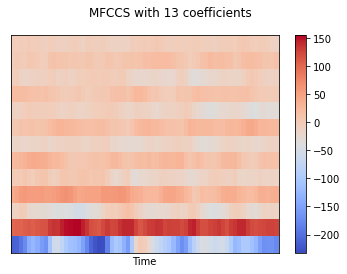
\includegraphics{img/3/mfcc.png}
    \caption{MFCC de un fragmento de 30s de una canción. Extraído de spotmyfm/Ludwig/notebooks/gtzan/mfcc.ipynb}
    \label{fig:MFCC}
\end{figure}
Los coeficientes cepstrales en las frecuencias de mel o MFCC Fig.\ref{fig:MFCC} son un tipo
de representación de la densidad espectral del sonido que intentan
representar la percepción auditiva humana.

Son muy utilizados en tareas de reconocimiento del habla y recuperación
de información musical.

Estos coeficientes están ajustados sobre la \textbf{escala de mel}, una
escala que aproxima la escala de tono a una escala similar a la
percepción humana, mejorando la representación del sonido.

Para obtener los MFCC partimos del espectrograma de mel, un
espectrograma ajustado a la escala de mel. En este caso, estamos
intentando obtener el espectrograma de un espectrograma, también conocido como cepstrum.

Un método para calcular los MFCCs puede\footnote{Cada biblioteca tiene una aproximación diferente.} ser el siguiente:

\begin{enumerate}
\def\labelenumi{\arabic{enumi}.}
\item
  Separar la señal en segmentos (hop\_length)
\item
  Aplicar la Transformada Discreta de Fourier a cada segmento para
  obtener la \textbf{potencia espectral}.
\item
  Transformar los resultados del paso 2 a la escala de mel.
\item
  Aplicar el logaritmo a cada frecuencia de mel, (escala logarítmica en
  \textbf{decibelios}).
\item
  Aplicar la Transformada Discreta del Coseno al resultado del paso 4
\item
  Escoger $N$ MFFCs\footnote{En \ref{fig:MFCC} se han escogido $N=13$ MFCCs}.
\end{enumerate}

Los pasos 1-3 se corresponden con la obtención de un espectrograma de mel.

Se recomienda consultar el apéndice A de \cite{book_mfcc} para consultar los detalles de la extracción. 

\section{Clasificación mediante Redes Neuronales
Convolucionales}\label{clasificacion_cnn}

Las redes neuronales convolucionales son una de las arquitecturas
neuronales más utilizadas en visión artificial debido a su poder para detectar patrones en imágenes, en nuestro caso vamos a buscar patrones en una representación bidimensional del sonido, los MFCCs \ref{coeficientes-cepstrales-en-las-frecuencias-de-mel}. Estas redes suelen estar formadas por una serie de bloques
convolucionales, seguidos de una o varias capas densas en la salida de
la red, como muestra \ref{fig:bloque_conv}.
La zona aizquierda de la línea discontinua roja compone la parte convolucional de la red, mientras que a la derecha de la línea se encuentra la parte densa de la red. Las última capa densa, compuesta por 3 neuronas, hace referencia a la capa de salida. 

\begin{figure}[h]
\centering
\label{fig:bloque_conv}
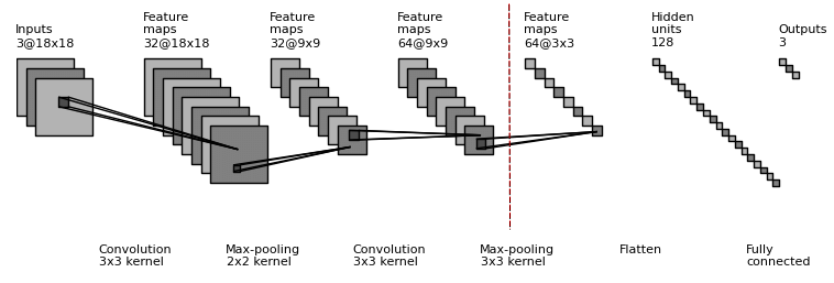
\includegraphics[width=2.99679in,height=1.01667in]{img/memoria/3/cnn.png}
\caption{Arquitectura de una red convolucional. Extraído de \cite{CNN_architecture} }
\end{figure}
\hypertarget{bloque-convolucional}{%
\subsection{Bloque Convolucional}\label{bloque-convolucional}}

Estos bloques, formados por capas, buscan resaltar los elementos más
relevantes en los datos a partir de las
operaciones de convolución y pooling.

La operación de convolución está formada por un kernel o filtro Fig.\ref{fig:kernel} que se
aplica Fig.\ref{fig:cnn_operation} a través de los datos. En el caso de la capa de convolución, los
pesos entrenables de dicha capa son el propio kernel.

\begin{figure}
    \centering
    \label{fig:kernel}
    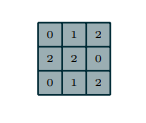
\includegraphics{img/memoria/3/kernel.png}
    \caption{Kernel 3x3. Extraído de \cite{convolution_guide}}
\end{figure}

Esta operación puede estar acompañada por una función de activación para
cada una de las neuronas, como por el ejemplo la función de activación
RELU \eqref{eq:relu_cnn}.

\begin{equation}
    \label{eq:relu_cnn}
    Relu(x) = max(0,x)
\end{equation}

\begin{figure}
    \centering
    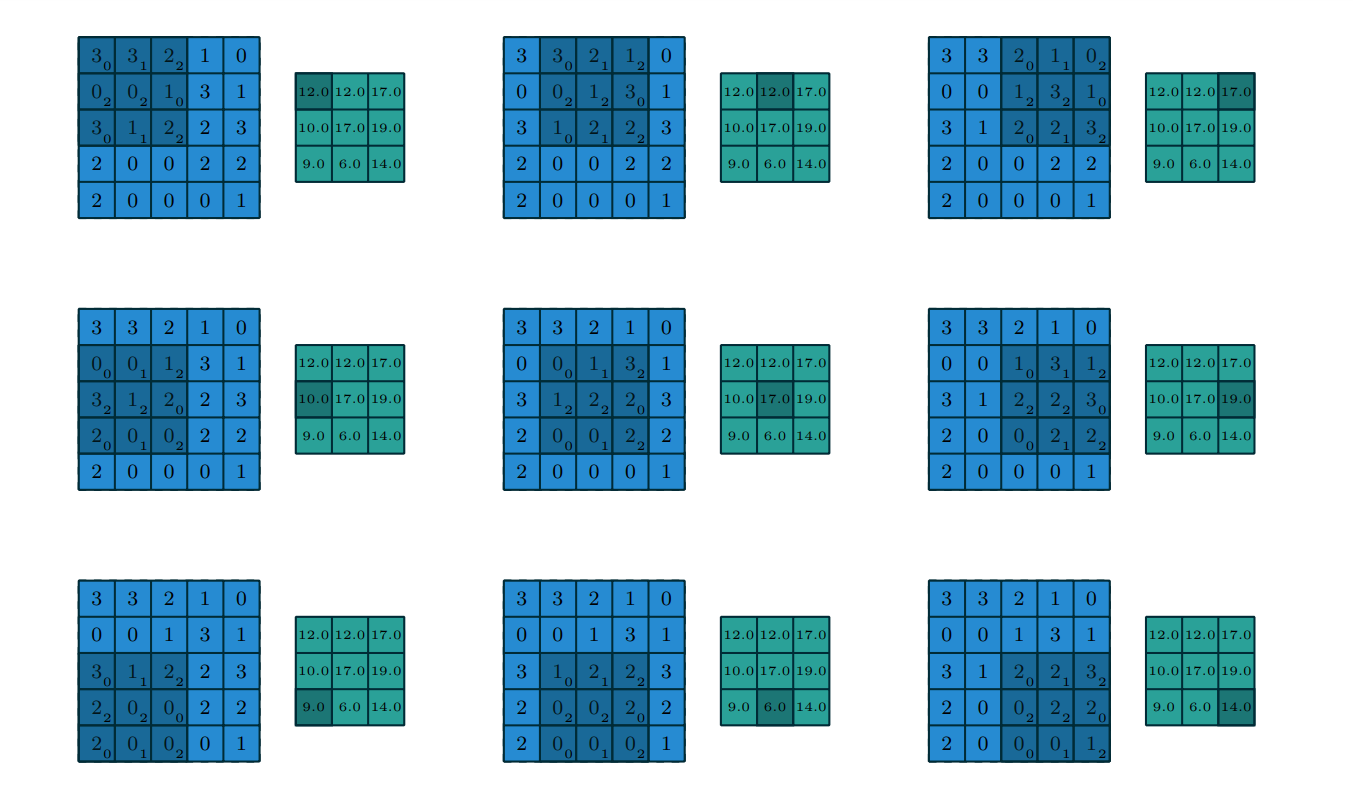
\includegraphics[width=5.90556in,height=3.52639in]{img/memoria/3/convolution.png}
    \caption{Aplicación del kernel 3x3 sobre un área 5x5. Extraído de \cite{convolution_guide}}
    \label{fig:cnn_operation}
\end{figure}

Por otro lado, la operación de pooling intenta reducir el tamaño de la
entrada, dejando solo los datos relevantes de un área. Se aplica de la
misma manera que una convolución, pero en vez de aplicar un kernel,
realizamos una operación aritmética sobre el área, como obtener el valor
más grande del área (Max Pooling) o la media de todos los valores
(Average Pooling)

Un bloque convolucional puede contener otras capas, como capas de
normalización, que normalizan de nuevo los datos para trabajar siempre
en el intervalo {[}0,1{]} o [-1, 1].

\hypertarget{densa}{%
\subsection{Densa}\label{densa}}

La salida de una red neuronal puede estar formada por capas densas, estas capas
tienen una entrada unidimensional, por lo que si la salida del último
bloque convolucional no es unidimensional, es necesario utilizar una
operación de Flatten que transforma la matriz de entrada en una única
fila concatenando cada una de las filas de la matriz.\\
En este tipo de arquitectura, cada una de las neuronas de una capa se interconectan con todas las neuronas de la capa siguiente. 

Cada neurona está formada por:

\begin{itemize}
\item
  Entradas ($[x_1 \dots x_n]$)
\item
  Salida  ($y$)
\item
  Vector de pesos entrenables ($[w_1 \dots w_n]$)
\item
  Función de activación ($fn(x)$)
\item
  Bias de activación entrenable ($[b_1 \dots b_n]$)
\end{itemize}

Y la salida (o salidas) de una neurona se calculan de la siguiente manera \eqref{eq:densa}.
\begin{equation}
    \label{eq:densa}
    y = fn(x \cdot w + b)
\end{equation}

La salida de cada una de estas neuronas se propaga a la siguiente capa como la entrada de cada neurona.

\hypertarget{capa-de-salida}{%
\subsection{Capa de Salida}\label{capa-de-salida}}

En tareas de clasificación, la capa de salida está formada por una o
varias neuronas \footnote{Depende del número de clases a clasificar}, y una función de
activación. Si debemos clasificar \textbf{varias clases}, utilizamos la
función de activación Softmax, que aplica una normalización en la salida
para resaltar la salida con la clase resultante.

Conociendo la salida de cada una de las neuronas, obtenemos la neurona
con la salida más cercana a 1 (la salida más grande)
\begin{equation}
   \sigma(z_i) = \frac{e^{z_{i}}}{\sum_{j=1}^K e^{z_{j}}} \ \ \ for\ i=1,2,\dots,n
   \label{eq:softmax}
\end{equation}



Para obtener la clase, calculamos cual es la neurona con la activación más elevada.
\begin{equation}
    clase = argmax([y_0 \dots y_n])
\end{equation}



En tareas de clasificación con \textbf{varias etiquetas} (multietiqueta), utilizamos la
función de activación Sigmoide, que permite a cada neurona tener una
salida entre 0 y 1, siendo este la confianza de que la clase contenga
dicha etiqueta.

\begin{equation}
    sigmoid(x) =  \frac{\mathrm{1} }{\mathrm{1} + e^-x }
    \label{eq:sigmoid}
\end{equation}    

Consideramos que una entrada contiene una etiqueta si el resultado de la sigmoide es mayor o igual que 0.5.


\hypertarget{cuantizacion-de-redes-neuronales}{%
\section{Cuantización de Redes
Neuronales}\label{cuantizacion-de-redes-neuronales}}

La cuantización de redes neuronales es una de las técnicas de
optimización de redes neuronales entrenadas más utilizada.\\
El proceso de cuantización consiste en convertir los distintos pesos (y
por tanto operaciones) de la red neuronal a un tipo de datos con menos
bits, lo que permite ahorrar memoria y acelerar las operaciones.
Normalmente, la cuantización convierte los tensores de FLOAT32 (4 bytes
por peso) a INT8 (1 byte por peso).

\begin{figure}
    \centering

    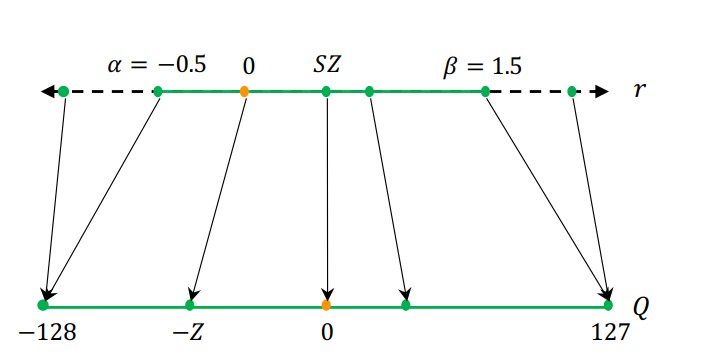
\includegraphics[width=5in,height=2.46875in]{img/3/quant.png}
    \caption{Cuantización INT8 en el intervalo $[-0.5,1.5$]. Extraído de \cite{quant_survey}}
    \label{fig:quant}
\end{figure}

En el proceso de cuantización tenemos presente dos parámetros para cada
uno de los tensores:

\textbf{Escala ($S$)}: Es un número decimal que nos permite escalar los
valores entre un número real y uno cuantizado.

\textbf{Zero Point ($Z$):} Es un número dentro del intervalo de cuantización.
Nos indica el valor del 0 real en valores cuantizados.

Estos valores son calculados a partir de analizar las distribución de los distintos tensores y activaciones.

\begin{equation}
    S = \frac{\beta - \alpha}{\beta_q - \alpha_q}    
\end{equation}

\begin{equation}
    Z = \left\lceil\frac{\beta\alpha_q - \alpha\beta_q}{\beta-\alpha}\right\rfloor
\end{equation}



En el caso de la distribución de valores reales, debemos conocer el valor mínimo
($\alpha$) y el máximo ($\beta$) del tensor/distribución a cuantizar.\footnote{Existen otras técnicas más avanzadas que tienen en cuenta la existencia de outliers en la distribución, lo que puede aumentar el ruido de cuantización.} 

Para los tensores cuantizados, $\alpha_q$ y $\beta_q$ se corresponden con el mínimo y el máximo de
los tipos de datos, para INT8,  $\alpha_q = -128$ y $\beta_q = 127$.

Una vez obtenidos $S$, $Z$, $\alpha_q$ y $\beta_q$, ya podemos cuantizar o decuantizar los distintos tensores con la siguiente ecuación.\footnote{La operación de decuantización debe tener en cuenta los errores de redondeo y clip si se quiere recuperar $x$. Nosotros no tenemos en cuenta los errores ya que no afectan al rendimiento de la red.}
\begin{equation}
    x_q = clip(round(\frac{1}{s}x + z), \alpha_q, \beta_q)
\end{equation}


Siendo clip una operación de saturación que impide que resultado de la cuantización sea un valor sea menor que $\alpha_q$ o mayor que $\beta_q$.
En la figura \ref{fig:quant} esta operación se ve reflejada en los valores que están fuera del intervalo $[\alpha,\beta]$


\hypertarget{tecnicas-de-cuantizacion}{%
\subsection{\texorpdfstring{Técnicas de Cuantización
}{Técnicas de Cuantización }}\label{tecnicas-de-cuantizacion}}
Existen dos técnicas de cuantización post entrenamiento:
\subsubsection{Fake Quantization o Cuantización Dinámica:}
Los pesos se almacenan en un tipo de datos inferior, pero los parámetros
de cuantización $S$ y $Z$ se calculan en tiempo de inferencia.
\subsubsection{Fixed Quantization:}
En este caso los parámetros de la cuantización se calculan durante el
proceso de cuantización. Este tipo de cuantización requiere utilizar un
\textbf{conjunto de datos representativo} \textbf{de entrada} durante el
proceso de cuantizado, con el que se calcularán los parámetros de
cuantización de cada tensor.

\hypertarget{resultados-de-la-cuantizaciuxf3n}{%
\subsection{Resultados de la
cuantización}\label{resultados-de-la-cuantizaciuxf3n}}
\begin{figure}
    \centering
    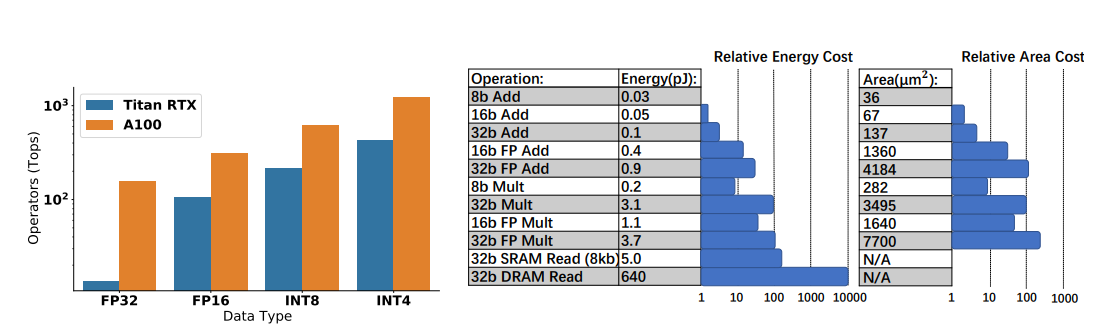
\includegraphics[width=5in,height=1.45833in]{img/3/quant_res.png}
    \caption{Resultados del coste de la operaciones dependiendo del tipo de dato de una red neuronal. Extraído de \cite{quant_survey}}
    \label{fig:quant-res}
\end{figure}

Si bien este proceso es muy eficiente como se puede observar en la figura \ref{fig:quant-res}, tiene un inconveniente muy
importante, y es que la salida de una neurona está limitada a tantos
valores como como el tipo de dato que utilicemos. En el caso de INT8 o UINT8, una neurona solo puede tener 256 valores distintos en su salida.

Por otro lado, esto no debería ser ningún problema si trabajamos con
tareas de clasificación con pocas etiquetas, pero es importante comprobar con un conjunto de
prueba que la precisión de la red no se ha visto afectada por la
cuantización.


\hypertarget{ensembles-ova-y-ovo}{%
\section{Ensembles, OVA y OVO}\label{ensembles-ova-y-ovo}}

Existen múltiples técnicas para clasificar conjuntos de datos con múltiples
clases. En este aparatado vamos a comentar dos tipos de ensembles que
unen varios clasificadores binarios para obtener un único clasificador
multiclase.
En algunas situaciones, los ensembles binarios pueden ser mucho más robustos que un único clasificador multietiqueta. 
Hemos planteado el uso de ensembles para mejorar el rendimiento de los distintos clasificadores de clasificación de géneros y estados de ánimo.

\begin{figure}[h]
    \centering
    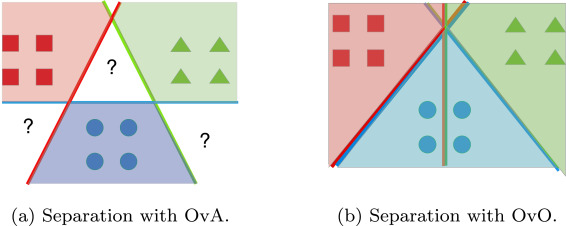
\includegraphics[]{img/3/ova-ovo.jpg}
    \caption{Comparación entre OVA y OVO. Extraído de \cite{OVA_vs_OVO}}
    \label{fig:ova-ovo}
\end{figure}


\hypertarget{one-vs-all}{%
\subsection{One vs All}\label{one-vs-all}}

El ensemble One vs All (OVA) divide un problema con $N$ clases en $N$
clasificadores binarios. Cada uno de estos clasificadores se encarga de
identificar si una entrada se corresponde con una clase (1) o no (0). En
este caso, es importante que el clasificador no esté calibrado, es decir,
su salida debe asemejarse con la confianza del resultado, ya que, si nos
encontramos con un conflicto entre varios clasificadores base por tener
la misma salida, no vamos a poder predecir la clase correctamente.

\textbf{Ejemplo Red Neuronal Binaria}

Si utilizamos la \textbf{función de activación escalón} en la neurona de
salida de nuestra red neuronal, nos encontramos con que la salida
únicamente tiene dos valores, 0 y 1, por lo que no conocemos la
confianza de la predicción.

Por otro lado, si utilizamos la \textbf{función sigmoide} \eqref{eq:sigmoid} como función
de activación, nos encontramos con una función cuyo recurrido son
valores reales en el intervalo {[}0, 1{]}, por lo que podríamos
considerar que la salida es la confianza que tiene la red ante una
predicción.

\hypertarget{one-vs-one}{%
\subsection{One vs One}\label{one-vs-one}}

El ensemble One vs One (OVO), a diferencia del ensemble OVA, busca una
clasificación más robusta entrenando un mayor número de clasificadores\\
Si en el ensemble OVA únicamente lidiábamos con las colisiones teniendo en cuenta
la confianza, el ensemble OVO es capaz de conocer si un dato pertenece a
una clase o a otra, ya que cada uno de los clasificadores se entrena con
un subconjunto de datos formado solo por dos clases\footnote{Clasificación Binaria}.

En este caso, tenemos que entrenar $L = K(K-1)/2$ clasificadores binarios,
un número mucho más grande que en el ensemble OVA, por lo que el coste
en memoria y tiempo de entrenamiento es mucho mayor.

En el caso del ensemble OVO, el clasificador base no solo no tiene que
estar correctamente calibrado, sino que además las salidas deben estar
comprendidas en el intervalo {[}-1, 1{]}, siendo -1 la clase A, 1 la
clase B, y 0 el valor correspondiente la clase desconocida.

Para evaluar la salida de todos los clasificadores, debemos construir
una matriz $N \times L$ (\ref{fig:matrix-ovo}), que permita convertir el vector $L$ a un vector con $N$
elementos con la confianza de cada clase. Cada fila de la matriz se
corresponde con cada clase, y debemos asignar el mismo valor (1 o -1)
que hemos utilizado como etiqueta durante el entrenamiento
\begin{figure}[h]
    \centering
    $$
    M = 
    \begin{bmatrix}
    1 & 1 & 1 & 0 & 0 & 0 \\
    -1 & 0 & 0 &  1 & 1 & 0 \\
    0 & -1 & 0 & -1 & 0 & 1 \\
    0 & 0 & -1 & 0 & -1 & -1 
    
    \end{bmatrix}
    $$
    \label{fig:matrix-ovo}
    \caption{Matriz para N=4}
\end{figure}


Haremos una multiplicación de matrices entre la matriz y la salida de
los clasificadores, obteniendo una matriz N x L con la probabilidad de
cada clase. Como hemos utilizado valores en el intervalo {[}-1, 1{]}
como salida de cada clasificador, al realizar la multiplicación de
matrices nos encontraremos con que únicamente tenemos valores positivos.\\
Si sumamos todas las columnas, de la matriz anterior obtendremos la
confianza del ensemble para cada uno de los datos.


\section{Ball Tree}\label{ball_tree}
Un ball tree o árbol de bolas es una estructura de datos jerárquica utilizada para la gestión de vecindarios de instancias. Esta estructura de datos permite conocer de una manera eficiente el vecindario de una instancia.

Se ha utilizado esta estructura de datos para buscar los vecinos más cercanos a una canción, como una posible técnica para identificar canciones similares.

Para construir un árbol de bolas, las instancias se dividen en dos clusters o bolas\footnote{También conocido como esferas o hiperesferas}, siendo cada cluster una rama del árbol. Los cluseters son calculados de la siguiente manera:
\begin{enumerate}
    \item Se selecciona una instancia aleatoria
    \item Se busca la instancia más alejada a la instancia seleccionada
    \item Se calcula el punto intermedio que hay entre las dos instancias
    \item Se divide el espacio en dos mediante un hiperplano
    \item Se calculan los centroides de los clusters que hay en cada división.
    \item Se crea una esfera que cubra todos las instancias de cada clúster
\end{enumerate}\\
Repetimos el proceso para cada una de las esferas hasta alcanzar el número de instancias por hoja buscado (Por defecto son 40 instancias por hoja en SKLearn).

Hecho esto, podemos consultar rápidamente el vecindario correspondiente a una nueva instancia a partir de los centroides más cercanos a nuestra instancia, sin necesidad de explorar todos los vecinos posibles. 

\section{Sistemas de Recomendación}
Un sistema de recomendación es un algoritmo que intenta predecir la valoración o interés que puede tener un usuario ante un nuevo elemento. Existen dos tipos principales de sistemas de recomendación, los sistemas basados en contenido y los filtrados colaborativos. 

Los sistemas basados en contenido realizan recomendaciones a partir de las etiquetas o metadatos del elemento. Se ha usado este tipo de sistema de recomendación para recomendar canciones similares basados en características extraídas del audio de las canciones. Se ha explorado el uso de estos sistemas en el apartado \ref{recomend_contenido}.

Los sistemas colaborativos tienen en cuenta las valoraciones o gustos de otros usuarios para realizar las recomendaciones.
Estos sistemas funciona a partir de la creación de una matriz usuario/elemento, en la que se almacena las valoraciones de los usuarios. De esta matriz se puede extraer una matriz usuario/usuario con la similitud que hay entre los gustos de los distintos usuarios. Para estos sistemas de filtrado se recomienda usar Suprise \ref{scikit-surprise}, una biblioteca que implementa una gran variedad de algoritmos para trabajar con sistemas colaborativos. Se ha usado este sistema de recomendación para rellenar playlists de usuario, como explora el apartado \ref{recomend_colab}.